\def\year{2019}\relax
%File: formatting-instruction.tex
\documentclass[letterpaper]{article} %DO NOT CHANGE THIS
\usepackage{aaai19}  %Required
\usepackage{times}  %Required
\usepackage{helvet}  %Required
\usepackage{courier}  %Required
\usepackage{url}  %Required
\usepackage{graphicx}  %Required
\frenchspacing  %Required
\setlength{\pdfpagewidth}{8.5in}  %Required
\setlength{\pdfpageheight}{11in}  %Required

\usepackage{amssymb}
\usepackage{amsmath,amsthm}
\usepackage{float}
\usepackage{url}
\usepackage{setspace}
\usepackage{hyperref}
\usepackage{todonotes}
\usepackage{amsthm} 
\usepackage[ruled,vlined,linesnumbered]{algorithm2e} 
\usepackage{makecell}
\usepackage{upgreek}
\onehalfspacing
\usepackage{pdfpages}
\usepackage{times}
\usepackage{multirow}
\usepackage[toc,page]{appendix}
\usepackage{listings}
\newtheorem{thm}{Theorem}
\newtheorem{lemma}[thm]{Lemma}
\newtheorem{definition}[thm]{Definition}
\newtheorem{observation}[thm]{Observation}
\newtheorem{theorem}[thm]{Theorem}
\newtheorem{claim}[thm]{Claim}
\newtheorem{example}[thm]{Example}
\newtheorem{proposition}[thm]{Proposition}
\newtheorem{corollary}[thm]{Corollary}
\usepackage{color,soul}
\usepackage{tikz}
\usetikzlibrary{arrows,shapes.geometric,shapes.arrows}
\usepackage{pgfplots}
\usepackage{multirow}


\DeclareMathOperator{\supp}{support}
\DeclareMathOperator{\support}{support}
\DeclareMathOperator{\Trim}{Trim}
\DeclareMathOperator{\LTrim}{LTrim}
\SetKwFunction{mEqOne}{mEqOne} 
\DeclareMathOperator{\KlmApprox}{Approx}
%\DeclareMathOperator{\OptTrim}{KolmogorovApprox}
\DeclareMathOperator{\OptTrim}{OptTrim}


  \pdfinfo{
	/Title (Deadline estimation by using an optimal approximation of discrete random variables with respect to the Kolmogorov distance
	)
	/Author ()}
\setcounter{secnumdepth}{0} 


\begin{document}


\title{Optimal Approximation of Discrete Random Variables \\ for Estimation of Probabilities of Missing Deadlines}
\author{}
\maketitle
\begin{abstract}
We present an efficient algorithm that, given a discrete random variable $X$ and a number $m$, computes a random variable whose support if of size at most $m$ and whose Kolmogorov distance from $X$ is minimal. We present the algorithm, analyse its correctness and computational complexity, and present a detailed empirical evaluation that shows how it performs in practice. The main application that we examine, which is our motivation for this work, is estimation of the probability missing deadlines in series-parallel schedules. Since exact computation of these probabilities is NP-hard, we propose to use the algorithm described in this paper to obtain an approximation.   
\end{abstract}


\section{Introduction}


Various approaches for approximation of probability distributions are studied in the literature~\cite{AMCR83,pavlikov2016cvar,PS77,vidyasagar2012metric,cohen2015estimating,CohenGW18}. 
These approaches vary in the types random variables considered, how they are represented, and in the criteria used for evaluation of the quality of the approximations. In this paper we propose an approach for compressing the probability mass function of a random variable $X$ such that the errors added to queries such as $Pr(X\leq t)$, for  any $t>0$, is minimal. In other words, we minimise the Kolmogorov distance between the approximation and the original random variable. Our motivation for this is estimation of the probability for missing deadlines, as described, e.g.,in~\cite{cohen2015estimating} and in~\cite{Kashef18}. Specifically, when $X$ represents the probability distribution of the time to complete some complex schedule and we cannot afford to maintain the full table of its probability mass function, we propose an algorithm for producing a smaller table, whose size can be specified, such that probabilities for missing deadlines are preserved as much as possible. 

The main contribution of this paper is an efficient algorithm for computing the best possible approximation of a given random variable with a random variable whose size is not above a prescribed threshold, where the measures of the quality of the approximation and of its size are as specified in the following two paragraphs. 

The case study examined in this paper is the problem of task trees with deadlines~\cite{cohen2015estimating,CohenGW18}. Hierarchical planning is a well-established field in AI~\cite{thomas1988hierarchical,erol1994htn,erol1996complexity}, and is still relevant nowadays~\cite{alford2016hierarchical,xiao2017hierarchical}. A hierarchical plan is a method for representing problems of automated planning in which the dependency among tasks can be given in the form of networks, here we focus on hierarchical plans represented by task trees. The leaves in a task tree are \emph{primitive} actions (or tasks), and the internal nodes are either \emph{sequence} or \emph{parallel} actions. The plans we deal with are of stochastic nature, and the task duration is described as probability distributions in the leaf nodes. We assume that the distributions are independent but {\em not} necessarily identically distributed and that the random variables are discrete and have a finite support. 

A sequence node denotes a series of tasks that should be performed consecutively, whereas a parallel node denotes a set of tasks that begin at the same time. A \emph{valid} plan is one that is fulfilled before some given \emph{deadline}, i.e., its \emph{makespan} is less than or equal to the deadline. The objective in this context is to compute the probability that a given plan is valid, or more formally computing $P(X<T)$, where $X$ is a random variable representing the makespan of the plan and $T$ is the deadline. The problem of finding the probability that a task tree satisfies a deadline is known to be NP-hard~\cite{mohring2001scheduling}. In fact, even the problem of summing a set of random variables is NP-hard~\cite{mohring2001scheduling}. This is an example of an explicitly given random variable that we need to estimate deadline meeting probabilities for.

We measure the quality of an approximation scheme by the distance between random variables and their approximations. Specifically, we use the Kolmogorov distance which is  commonly used for comparing random variables in statistical practice and literature. Given two random variables $X$ and $X'$ whose cumulative distribution functions (cdf) are $F_X$ and $F_{X'}$, respectively, the Kolmogorov distance between $X$ and $X'$ is $d_K(X,X')= \sup_t |F_X(t) - F_{X'}(t)|$ (see, e.g.,~\cite{gibbons2011nonparametric}). We say that $X'$ is a good approximation of $X$ if $d_K(X,X')$ is small. This distance is the basis for the often used Kolmogorov-Smirnoff test for comparing a sample to a distribution or two samples to each other. 

The size of a random variable is measured here by the size of its support, the set of possible outcomes, $|X|=|X|=|\{x\colon Pr(X=x) \neq 0\}|$. When probability mass functions are maintained as explicit tables, as done in many implementations of statistical software, the size of the support of the variable is proportional to the amount of memory needed to store it and to the complexity of the computations that manipulate it. 

Together, the exact notion of optimality of the approximation targeted in this paper is:
\begin{definition}
	A random variable $X'$ is an optimal $m$-approximation of a random variable $X$ if $|X'| \leq m$ and there is no random variable $X''$ such that $|X''| \leq m$ and $d_K(X,X'') < d_K(X,X')$.
\end{definition}

In these terms, the main contribution of the paper is an efficient (polynomial time and memory) algorithm that takes $X$ and $m$ as parameters and constructs an optimal $m$-approximation of $X$.

The rest of the paper is organised as follows. In Section~\ref{sec:relwork} we describe how our work relates to other algorithms and problems studied in the literature. In Section~\ref{sec:alg} we detail the proposed algorithm, analyse its properties, and prove the main theorem. In Section~\ref{sec:exp} we demonstrate how the proposed approach performs on the problem of estimating the probability of missing deadlines in series-parallel schedules on randomly generated random variables and compare it to alternative approximation approaches from the literature. The paper is concluded with a discussion and with ideas for future work in Section~\ref{sec:discussion}.

%%%%%%%%%%%%%%%%%%%%%%%%%%%%%%%%%%%%%%%%%%%%%%%%%%%%%%%%%%%%%%%%%%%%%%%%%%%%%%%%%%%%%%%%%%%%
\section{Related work}\label{sec:relwork}
The most relevant work related to this paper is the papers on approximations of random variables in the context of estimating deadlines~\cite{cohen2015estimating,CohenGW18}. In these papers, $X'$ is defined to be a good approximation of $X$ if $F_{X'}(t) > F_{X}(t)$ for any $t$ and $\sup_t F_{X'}(t) - F_{X}(t)$ is small. Note that this measure is not a proper distance measure because it is not symmetric. The motivation given in these papers for using this type of approximation is for cases where overestimation of the probability of missing a deadline is acceptable but underestimation is not. In Section~\ref{sec:exp}, we consider the same case-studies examined by Cohen et al. and show how the algorithm proposed in this paper performs relative to the algorithms proposed there when both over- and under- estimations are allowed. As expected, the Kolmogorov distance between the approximated and the original random variable is considerably smaller when using the algorithm proposed in this paper. 

In the technical level, the problem we study in this paper is similar to the problem of approximating a set of 2-D points by a step function. The study of this problem was motivated by query optimisation and histogram constructions in database management systems~\cite{applf12,applf13,applf14,applf17,applf18,Fournier2011} and computational geometry~\cite{diaz2001fitting,fournier2008fitting}. There are, however, two technically significant differences between the problem studied in the context of databases and the problem we analyse in this paper. The first difference is that in the context of approximation of random variables, the step function (which is the cumulative distribution function in our context)  must end with a value one, since we are dealing with random variables which sums to one. The second difference is that the first step is not counted because there is no need to put a value in the support of the approximated random variable to generate this first step. These cannot be addressed by adding a constant (two) to $m$ because the first step is always present and because the requirement to end with the value one, restricts the set of eligible step functions. See Section~\ref{sec:alg} for more details.

Another relevant prior work is the theory of Sparse Approximation (aka Sparse Representation) that deals with sparse solutions for systems of linear equations, as follows. 
Given a matrix $D \in \mathbb{R}^{n \times p}$ and a vector $x \in \mathbb{R}^n$, the most studied sparse representation problem is finding the sparsest possible representation $\alpha \in \mathbb{R}^p$ satisfying $x = D\alpha$:
\[
\min_{\alpha \in \mathbb{R}^p} \|\alpha\|_0 \text{ subject to } x = D\alpha
\]
where $\|\alpha\|_0 = |\{ i \in [p]: \alpha_i \neq 0 \}|$ is the $\ell_0$ pseudo-norm, counting the number of non-zero coordinates of $\alpha$. This problem is known to be NP-hard with a reduction to NP-complete subset selection problems.
In these terms, using also the $\ell_\infty$ norm that represents the maximal coordinate and the $\ell_1$ norm that represents the sum of the coordinates, our problem can be phrased as:
\[
\min_{\alpha \in [0,\infty)^p}\|x - D\alpha\|_{\infty} \text{ subject to }  \|\alpha\|_0 = m \text{ and } \|\alpha\|_1=1
\]
where $D$ is the lower unitriangular matrix, $x$ is related to $X$ such that the $i$th coordinate of $x$ is $F_X(x_i)$ where $\support(X)=\{x_1 < \cdots < x_n\}$ and $\alpha$ is related to $X'$ such that the $i$th coordinate of $\alpha$ is $f_{X'}(x_i)$. The functions $F_X$ and $f_{X'}$ represent, respectively, the cumulative distribution function of $X$ and the mass distribution function of $X'$, i.e.,  the coordinates of $x$ are positive and monotonically increasing and its last coordinate is one. We show that this specific sparse representation problem can be solved in $O(n^2m)$ time and $O(m^2)$ memory.

%The presented work is also related to the research on binning in statistical inference. Consider, for example, the problem of credit scoring~\cite{zeng2017comparison} that deals with separating good applicants from bad applicants where the Kolmogorov–Smirnov statistic KS is a standard measure. The KS comparison is often preceded by a procedure called binning where small values in the the probability mass function are moved to nearby values. There are many methods for binning~\cite{mays2001handbook,refaat2011credit,bolton2010logistic,siddiqi2012credit}.
%In this context, our algorithm can be considered as a binning strategy that provides optimality guarantees with respect to the Kolmogorov distance.

Our study is also related to the work of Pavlikov and Uryasev~\cite{pavlikov2016cvar}, where a procedure for producing a random variable $X'$ that optimally approximates a random variable $X$ is presented. Their approximation scheme, achieved using linear programming, is designed for a different notion of distance called CVaR. The contribution of the present work in this context is that our method is direct, not using linear programming, thus allowing tighter analysis of time and memory complexities. Also, our method is designed for minimising the Kolmogorov distance that is more prevalent in applications. For comparison, in Section~\ref{sec:exp} we briefly discuss the performance of linear programming approach similar to the one proposed in~\cite{pavlikov2016cvar} for the Kolmogorov distance and compare it our algorithm. 

A problem very similar to ours is termed ``order reduction'' by Vidyasagar in~\cite{vidyasagar2012metric}. There, the author defines an information-theoretic based distance between discrete random variables and studies the problem of finding a variable whose support is of size $m$ and its distance from $X$ is as small as possible (where $X$ and $m$ are given). The only difference between this and the problem studied in this paper, is that Vidyasagar examines a different notion of distance. Vidyasagar proves that computing the distance (that he considers) between two probability distributions, and computing the optimal reduced order approximation, are both NP-hard problems, because they can both be reduced to nonstandard bin-packing problems. He then develops efficient greedy approximation algorithms. In contrast, our study shows that there are efficient solutions to these problems when the Kolmogorov distance is considered. 

%%%%%%%%%%%%%%%%%%%%%%%%%%%%%%%%%%%%%%%%%%%%%%%%%%%%%%%%%%%%%%%%%%%%%%%%%%%%%%%%%%%%%%%%%%%%
\section{An algorithm for optimal approximation}\label{sec:algEfficient}
In the scope of this section, let $X$ be a given random variable with a finite support of size $n$, and let  $0<m\leq n$ be a given complexity bound. The section evolves by presenting two algorithms for finding an optimal $m$-approximation of $X$. The first algorithm is $binsearchApprox(X,m)$ (Algorithm~\ref{alg:naive}) which runs in time of $O(n^2log(n))$ and the second one $linApprox(X,m)$ (Algorithm~\ref{alg:linear}) which runs in time of $O(nlog(n))$. We present both $binsearchApprox(X,m)$ and $linApprox(X,m)$ since Algorithm~\ref{alg:linear} is based on Algorithm~\ref{alg:naive} but carry major run-time improvement.

We begin our dissection by presenting a useful fact that it is enough to limit our search to approximations $X'$s such that $\support(X') \subseteq \support(X)$:

\begin{lemma}\label{lem:supContained}
	For every random variable $X''$ there is a random variable $X'$ such that $\support(X') \subseteq \support(X)$ and $d_{K}(X,X')\leq d_{K}(X,X'')$.
\end{lemma}

\begin{proof}
	Let $\{x_1 <\cdots<x_n\} = \support(X)$, and let $x_0 = -\infty, x_{n+1}=\infty$. Consider the random variable $X'$ whose probability mass function is
	$f_{X'}(x_i) = P(x_{i-1} < X'' \leq x_i)$ for $i=1,\dots,n-1$,  $f_{X'}(x_n) = P(x_{n-1} < X'')$, and $F_{X'}(x)=0$ if $x\notin \support(X)$.  Since we only "shifted" the probability mass of $X''$ to the support of $X$, we have that $f_{X'}$ is a probability mass function and therefore $X'$ is well defined. 	
	By construction, $|F_{X}(x_i)-F_{X'}(x_i)| = |F_{X}(x_i)-F_{X''}(x_i)|$ for every  $0 <  i < n$. For $i=n$ we have $|F_{X}(x_n)-F_{X'}(x_n)| = |1-1|=0$.
	Since $|F_{X}(x)-F_{X'}(x)| = |F_{X}(x_i)-F_{X'}(x_i)|$ for every  $0\leq   i  \leq  n$  and $x_i<x<x_{i+1}$, we have that $d_K(X,X')=max_{i}|F_{X}(x_i)-F_{X'}(x_i)|\leq max_{i}|F_{X}(x_i)-F_{X''}(x_i)|\leq d_K(X,X'')$.
\end{proof} 

Both of the algorithms presented in this section are using the dual problem in order to find the optimal $m$-approximation of $X$. The dual problem is: given a random variable $X$ with $|X| = n$, and some $0 \leq \varepsilon \leq 1$, find a new random variable $X'$ such that $|X'|\leq m$ where $0< m \leq n$ and $d_K(X,X')$ is minimal. 

We do not assume anything about the representation of the random variable $X$ given as an input to the $dual(X,\varepsilon)$ algorithm. However, we transform the representation of every given $X$, to the form of sorted CDF as described in line 1 in the algorithm, which takes $O(nlog(n))$ run-time and has to done only once. The $dual(X,\varepsilon)$ gets as input a random variable $X$ and some $\varepsilon$, the random variable $X$ is represented as in line 1, $X_{CDF} =\{(x_i, c_i)\}_{i=1}^n$ such that $c_i = Pr(X \leq x_i)$ and $\supp(X)=\{x_1 <\cdots < x_n\}$. In lines 3-4 we perform a single pass over $X_{CDF}$ starting from index 1 to find the last index where the cumulative distribution function of $X$ is less than $\varepsilon$, this index is now $f$. In lines 5-6 in the algorithm we start from the last index of $X_{CDF}$ which is $n$, and in decreasing order seek for the last index where the cumulative distribution function of $X$ is less than $1-\varepsilon$, this index is now $l$. The last part of the algorithm is a pass on all elements in $X_{CDF}$ between the indices $f$ and $l$ in order to construct the $m$-approximation random variable of $X$, $X'$. In lines 9-10 we check if the difference between the first element in the current set of indices (which we call $b$) and the last element in the current set of indices (which we call $e+1$) is less that $2\varepsilon$. If yes, we add the pair $\{(x_{b}, (c_b+c_e)/2 - s) \}$ to the set $S$. Otherwise, we add one to the counter of $e$. Note, the reason we need $s$ is to return the random variable $X'$ in a PDF representation since our main motivation is sum of random variables, this part takes $O(n)$ run-time.



\begin{algorithm}
	\DontPrintSemicolon
	Let $\{(x_i, c_i)\}_{i=1}^n$ be such that $c_i = Pr(X \leq x_i)$ and $\supp(X)=\{x_1 <\cdots < x_n\}$.\;
    $f \gets 0$, $l \gets n$+1\; 
    \While{$c_{f +1} \leq \varepsilon$}{$f \gets f + 1$}

    \While{$c_{l -1} \geq  1-\varepsilon$}{$l \gets l -1$}

	$S \gets \emptyset$, $s \gets 0$,$b \gets f$, $e \gets f$\;
	\While{$e<l$}{
	    \While{$c_{e+1}-c_{b} \leq 2\varepsilon \wedge e+1 <l$}{$e \gets e+1$}
	    $S \gets S \cup \{(x_{b}, (c_b+c_e)/2 - s) \}$\;
        $s \gets  (c_b+c_e)/2$, $b \gets e+1$\;
	}
	$S \gets S \cup \{(x_{l}, 1 - s) \}$\;
    \Return{A r.v. $X'$ such that $Pr(X'{=}x)=c$ if there is $c$ such that $(x, c) \in S$ and $Pr(X'{=}x)=0$ otherwise.}
    	
    	
	
	\caption{$dual(X,\varepsilon)$}   
	\label{alg:dual}
\end{algorithm}


\SetKwRepeat{Do}{do}{while}
%which c? why -s? name without any meaning, cant understand

\begin{theorem}\label{the:complexityDual}
	The $dual(X,\varepsilon)$ algorithm runs in time $O(n)$, using $O(n)$ memory where $n=|X|$.
\end{theorem}
\begin{proof}
	This algorithm describes a single pass over the random variable $X$. Lines 3-4 and lines 5-6 are easy to follow, each takes $O(n)$ in the worst case. Lines 8-12 also describe one pass over $X$ since the counter $e$ is updated to $e+1$ at most $n$ times. All together we get run-time complexity of $O(3n)$ = $O(n)$. We are constructing the set $S$ which is of size $n$ in the worst case, therefore, memory complexity is also $O(n)$. 
\end{proof}

The first technique we present is the $binsearchApprox(X,m)$ algorithm which is based on the work done by D{\'i}az-B{\'a}nez and Mesa~\cite{diaz2001fitting}. There are couple of significant changes between our $binsearchApprox(X,m)$ algorithm and the algorithm suggested by D{\'i}az-B{\'a}nez and Mesa~\cite{diaz2001fitting} addressing the differences presented in the Related Work section~\ref{sec:relwork}. The algorithm $binsearchApprox(X,m)$ gets as input a random variable $X$ and some number $m$. Again, we do not mind the original representation of $X$ since we can transform it to a sorted CDF representation in $O(nlog(n))$ run-time as in line 1 which we call $X_{CDF}$. In lines 3-8 we compute all possible errors, in other words, all possible $d_{K}(X,X')$ such that $X'$ is an approximation of $X$ and $\support(X') \subseteq \support(X)$. The error is just the difference between the CDF values of every two elements in $X_{CDF}$. After computing the set $E$, we sort it (line 9) in order to perform a binary search in the last part of the algorithm. In lines 10-19 we perform a binary search over the set $E$, in every step of the binary search we run the $X' = dual(X,\varepsilon)$ algorithm. If the size of $|X'|>m$ then we know that the error $\varepsilon$ is too small and need to extend the search in the right side of $E$, if the size of $|X'|<m$ then we know that the error $\varepsilon$ is too big and need to extend the search in the left side of $E$, otherwise we found the correct $m$. We run the search twice to handle the extreme case where $m \notin \{\forall \varepsilon\in E: |dual(X,\varepsilon)|\}$ and return the smallest $m'$ closest to $m$.
 

\begin{algorithm}
	\DontPrintSemicolon
	Let $\{(x_i, c_i)\}_{i=1}^n$ be such that $c_i=Pr(X \leq x_i)$ and $\supp(X)=\{x_1 < \cdots < x_n\}$.\;
    $E \gets \emptyset$\; 
    \For{$i \gets 1$ \textbf{to} $n-1$}{
    	\For{$j \gets i+1$ \textbf{to} $n-1$}{
        		\If{$i=1$} {
                	$E \gets E \cup \{ c_j \}$
                }
        		$E \gets E \cup \{ (c_j-c_i)/2 \}$
        }
        $E \gets E \cup \{ 1 - c_i \}$
    }
    Let $e_1<\cdots<e_{n'}$ be such that $E=\{e_1,\dots,e_{n'}\}$ \;
    
    \For{$i \gets 1 \textbf{ to } 2$}{
        $l\gets 1$, $r \gets n'$, $k \gets 1$ \;
        \Do{$k \neq k'$}{
                $k' \gets k$,$k \gets \lceil (l + r)/2 \rceil$\;
        		$X' \gets dual(X,e_k)$, $m' \gets |X'|$\;
        		\lIf{$m' < m$}{
        		    $l \gets k$
        		}
                \lIf{$m' > m$}{
        		    $r \gets k-1$
        		}
                \lIf{$m' = m$}{
        		    $r \gets k$
        		}
        }
        $m \gets m'$\;
    }
    \Return{X'}

	\caption{$binsearchApprox(X,m)$}   
	\label{alg:naive}
\end{algorithm}

\begin{theorem}\label{the:complexityDual}
	The $binsearchApprox(X,m)$ algorithm runs in time $O(n^2log(n))$, using $O(n^2)$ memory where $n=|X|$.
\end{theorem}
\begin{proof}
	In the first part of the algorithm, lines 2-8, we construct the set $E$ which takes $O(n^2)$ run-time. In the second part of the algorithm, line 9, we sort the set $E$ which takes $O(n^2log(n^2)) = O(n^2log(n))$  run-time. The third part of the algorithm, lines 10-19, describes a binary sort over the set $E$ where in each step of the sorting we run the $dual$ algorithm, which takes $O(n log(n^2)) = O(n log(n))$ run-time. We run this part twice then we get $O(2n log(n))$. All together, the run-time complexity is $O(n^2+n^2log(n)+2n log(n)) = O(n^2log(n))$ and the memory complexity is for storing the set $E$ which is $O(n^2)$.
\end{proof}

As a step towards $linApprox(X,m)$ algorithm, we present the algorithm $saddlebackApprox(X,m)$ that takes $O(n^2)$ run-time, this technique is very similar to $linApprox(X,m)$ algorithm. The algorithm $saddlebackApprox(X,m)$ gets as input a random variable $X$ and some number $m$. Again, we represent $X$ as a sorted CDF in $O(nlog(n))$ run-time as in line 1 and call it $X_{CDF}$. In line 4 We describe implicitly the sorted matrix $E$, and in lines 3-7 we perform a search over this matrix, in every step of the search we run the $X' = dual(X,\varepsilon)$ algorithm. If the size of $|X'|>m$ then we know that the error $e$ is too small and need to extend the search in the lower side of the matrix, if the size of $|X'|<m$ then we know that the error $e$ is too big and need to extend the search in the right side of the matrix and store this $e$ in $S$. We store in set $S$ all possible candidates for the correct $e$ and in line 8 we get the maximal $m$ with the minimal $e$ value.


\begin{algorithm}
	\DontPrintSemicolon
	Let $\{(x_i, c_i)\}_{i=1}^n$ be such that $c_i=Pr(X \leq x_i)$ and $\supp(X)=\{x_1 < \cdots < x_n\}$.\;
    $i \gets 1$, $j \gets \lceil n/2 \rceil$, $S \gets \emptyset$\;

	\While{$i < \lfloor n/2 \rfloor + 1 \wedge j \geq 2$}
	{
% 		$ e \gets \begin{cases}
% 			c_j   & \text{if } i=\lfloor n/2 \rfloor+1; \\
% 			1-c_i & \text{if } j=\lceil n/2 \rceil; \\
% 			(c_{n+1-j} {-} c_i)/2  & \text{otherwise}
% 		\end{cases}$\;
		
		
		$X' \gets dual(X,e_{i,j})$, $m' \gets |X'|$\;
	
		\lIf {$m'  > m$}
		{
			$j \gets j - 1$
		}
		\lIf {$m' \leq m$} {
			$i \gets i + 1$, $S \gets S \cup (m',e)$			
		}
	}
	$e \gets \min\{e\colon (m',e) \in \underset{(m',e)\in S}{\operatorname{arg\,max}}\, m'\}$\;
	\Return{$dual(X,e)$}
	
	\caption{$saddlebackApprox(X,m)$}   
	\label{alg:saddleback}
\end{algorithm}


\begin{algorithm}
		\DontPrintSemicolon
		Let $\{(x_i, c_i)\}_{i=1}^n$ be such that $c_i=Pr(X \leq x_i)$ and $\supp(X)=\{x_1 < \cdots < x_n\}$.\;
		
		$w \gets 2^{\lceil \log_2(n/2) \rceil}$,
		$h \gets 2^{\lceil \log_2(n/2+1) \rceil}$ \;
				
		$S \gets  \{ ((1, 1)),(w,h)) \}$, $S' \gets \emptyset$\;
		
		
		\While{$S \neq S'$}
		{
			$S' \gets S$,
			$S \gets  \bigcup_{s \in S} split(s)$\;
			
			$e^- {\gets} median(\{ e_{i_1,j_1} \colon ((i_1,j_1),(i_2,j_2)) \in S \}) $\;		
			$e^+ {\gets} median(\{ e_{i_2,j_2} \colon ((i_1,j_1),(i_2,j_2)) \in S \}) $\;			

			\For{$ e \in \{ e^-,e^+ \}$} {
				$X' \gets dual(X,e)$, $m' \gets |X'|$\;
	
				\If {$m' \leq m$} {
					$S \gets$ $S \setminus \{ ((i_1,j_1),(i_2,j_2)) \in S \colon e_{i_1,j_1} > e \}$ \;
				}
			
				\Else %\If {$m'  > m$}
				{
					$S \gets$ $S \setminus \{ ((i_1,j_1),(i_2,j_2)) \in S \colon e_{i_2,j_2} \leq e \}$ \;
				}
			}
		}
	
		$S'' \gets \{(|dual(X,e_{i,j})|,e_{i,j}) \colon ((i,j),(i,j)) \in S\}$\;	
	
		$e \gets \min\{e\colon (m',e) \in \underset{(m',e)\in S''}{\operatorname{arg\,max}}\, m'\}$\;
		\Return{$dual(X,e)$}

		\caption{$linApprox(X,m)$}   
		\label{alg:linear}
	\end{algorithm}

	\begin{procedure}
		\DontPrintSemicolon
		$j^- \gets \lfloor (j_1+j_2)/2 \rfloor$,
		$j^+ \gets \lceil (j_1+j_2)/2 \rceil$\;
		$i^- \gets \lfloor (i_1+i_2)/2 \rfloor$,
		$i^+ \gets \lceil (i_1+i_2)/2 \rceil$\;

		\Return{\hspace{4cm}$
			\{ ((i_1, j_1), (i^-, j^-)),
			((i_1, j^+), (i^-, j_2))$,
			$((i^+, j_1), (i_2, j^-)),
			((i^+, j^+), (i_2, j_2))    \}$}
		
		\caption{{$split(((i_1,j_1),(i_2,j_2)))$}()}
		\label{proc:split}
	\end{procedure}
	
	
	
	Let 
	$$e_{i,j} = \begin{cases}
	c_j   & \text{if } i > n; \\
	1-c_i & \text{if } j \geq n; \\
	(c_{n+1-j} {-} c_i)/2  & \text{otherwise}.
	\end{cases}$$









%%%%%%%%%%%%%%%%%%%%%%%%%%%%%%%%%%%%%%%%%%%%%%%%%%%%%%%%%%%%%%%%%%%%%%%%%%%%%%%%%%%%%%%%%%%%
% \section{An algorithm for optimal approximation}\label{sec:alg}
% In the scope of this section, let $X$ be a given random variable with a finite support of size $n$, and let  $0<m\leq n$ be a given complexity bound. The section evolves by developing notations and by collecting facts towards an algorithm for finding an optimal $m$-approximation of $X$.

% The first useful fact is that it is enough to limit our search to approximations $X'$s such that $\support(X') \subseteq \support(X)$:

% \begin{lemma}\label{lem:supContained}
% 	For every random variable $X''$ there is a random variable $X'$ such that $\support(X') \subseteq \support(X)$ and $d_{K}(X,X')\leq d_{K}(X,X'')$.
% \end{lemma}

% \begin{proof}
% 	Let $\{x_1 <\cdots<x_n\} = \support(X)$, and let $x_0 = -\infty, x_{n+1}=\infty$. Consider the random variable $X'$ whose probability mass function is
% 	$f_{X'}(x_i) = P(x_{i-1} < X'' \leq x_i)$ for $i=1,\dots,n-1$,  $f_{X'}(x_n) = P(x_{n-1} < X'')$, and $F_{X'}(x)=0$ if $x\notin \support(X)$.  Since we only "shifted" the probability mass of $X''$ to the support of $X$, we have that $f_{X'}$ is a probability mass function and therefore $X'$ is well defined. 	
% 	By construction, $|F_{X}(x_i)-F_{X'}(x_i)| = |F_{X}(x_i)-F_{X''}(x_i)|$ for every  $0 <  i < n$. For $i=n$ we have $|F_{X}(x_n)-F_{X'}(x_n)| = |1-1|=0$.
% 	Since $|F_{X}(x)-F_{X'}(x)| = |F_{X}(x_i)-F_{X'}(x_i)|$ for every  $0\leq   i  \leq  n$  and $x_i<x<x_{i+1}$, we have that $d_K(X,X')=max_{i}|F_{X}(x_i)-F_{X'}(x_i)|\leq max_{i}|F_{X}(x_i)-F_{X''}(x_i)|\leq d_K(X,X'')$.
% \end{proof}

% %Next, note that every random variable $X''$ with support of size at most $m$ that is contained in $\support(X)$ can be described by first setting the (at most $m$) elements of the support of $X''$; then for every such option, determine $X''$ by setting probability values for the elements in the chosen support of $X'$, and setting $0$ for rest of the elements.

% For a set $S\subseteq \support(X)$, let $\mathbb{X}_S$ denote the set of random variables whose supports are contained in $S$. In Step 1 below, we identify a random variable in $\mathbb{X}_S$  that minimizes the Kolmogorov distance from $X$. We denote the Kolmogorov distance between this variable and $X$ by $\varepsilon(X,S)$. Then, in Step 2, we show how to efficiently find a set $S \subseteq \support(X)$ whose size is smaller or equal to $m$ that minimizes $\varepsilon(X,S)$. Then, in Step 3, an optimal $m$-approximation is constructed by taking a minimal approximation in $\mathbb{X}_S$ where $S$ is the set of size $m$ that that minimizes $\varepsilon(X,S)$. 

% \subsection*{Step 1: Finding an $X'$ in $\mathbb{X}_S$ that minimizes $d_K(X,X')$}


% We first fix a set $S\subseteq \support(X)$ and among all the random variables in $\mathbb{X}_S$ find one with a minimal distance from $X$. Denote the elements of $S$ in increasing order by $S=\{x_1<\dots<x_m\}$ and let $x_0=-\infty$ and $x_{m+1}=\infty$. Consider the following weight function:

% \begin{definition}\label{def:weight} For $0\leq i \leq m$ let
% 	\[
% 	w(x_i,x_{i+1})=
% 	\begin{cases}
% 	P(x_i < X < x_{i+1}) & \text{if $i=0$ or $i = m$;} \\
% 	P(x_i < X < x_{i+1})/2 & \text{otherwise.} \\	
% 	\end{cases}
% 	\]
% \end{definition}
% For each $1 <  i \leq m$ let $\hat x_i$ be the maximal element of $\support(X)$ that is smaller than $x_i$. 
% Note that, for $1\leq i \leq m$, $P(x_i < X < x_{i+1}) = F_X(\hat x_{i+1}) - F_X(x_i)$, a fact that we will use throughout this section.

% \begin{definition}\label{def:error}
% Let $\varepsilon(X,S) = \max\limits_{i=0,\dots,m} w(x_{i}, x_{i+1})$.
% \end{definition}



% We first show that $\varepsilon(X,S)$ is a lower bound for the distance between random variable in $\mathbb{X}_S$ and $X$. Then, we present a random variable $X'\in \mathbb{X}_S$ such that $d_K(X,X')=\varepsilon(X,S)$. It then follows that $X'$ is closets to $X$ in $\mathbb{X}_S$.

% %The intuition behind choosing these specific weights and $\varepsilon(X,S)$ being a lower bound is as follows.  Since for every $X'\in\mathbb{X}_S$ the probability mass of $X'$ for the elements not in $S$ are set to $0$, we have that $F_{X'}(\hat x_{i+1})=F_{X'}(x_i)$. Therefore the distance between $X'$ and $X$ at points $x_i$ and $\hat x_{i+1}$ that we have to take into additional account is increased by $F_X(\hat x_{i+1})-F_X(x_i) = P(x_i < X < x_{i+1})$.

% %Formally we have the following.

% \begin{proposition}\label{prop:minimal}
% 	If $X'\in\mathbb{X}_S$ then $d_K(X,X') \geq \varepsilon(X,S)$.
% \end{proposition}

% \begin{proof}
	
	
% 	By definition, for each $0\leq i\leq m$, $d_K(X,X') \geq \max \{|F_X(\hat x_{i+1}) - F_{X'}(\hat x_{i+1})|,|F_X(x_i) - F_{X'}(x_i)| \}$. Note that $F_{X'}(\hat x_{i+1})=F_{X'}(x_i)$ since the probability of  elements not in $S$ is  $0$.
	
% 	If $i=0$, that is $x_i=-\infty$, we have that $F_X(x_i)=F_{X'}(x_i)=F_{X'}(\hat x_{i+1})=0$ and therefore $d_K(X,X') \geq |F_X(\hat x_{i+1})| = |F_X(\hat x_{i+1}) - F_{X}(x_i)| =  P(x_i < X < x_{i+1})= w(x_i,x_{i+1})$.
	
% 	If $i =m$, that is $x_{i+1}=\infty$, we have that $F_X(\hat x_{i+1})=F_{X'}(\hat x_{i+1})=F_{X'}(x_i)=1$. 
% 	and therefore $d_K(X,X') \geq |1-F_X(\hat x_i)| = |F_X(\hat x_{i+1}) - F_{X}(x_i)| =  P(x_i < X < x_{i+1}) = w(x_i,x_{i+1})$. 
	
% 	%  we have that $F_X(x_i)=F_{X'}(x_i)=F_{X'}(\hat x_{i+1})=0$ 
% 	% 
% 	% 
% 	% 
% 	% We break the proof for the closed intervals where each support variable $x_i$ is a proper number, and for the open intervals where a support variable is either $-\infty$ or $\infty$.
	
% 	Otherwise for every $1\leq i< m$,  we use the fact that $max\{|a|,|b|\} \geq |a-b|/2$ for every $a,b\in\mathbb{R}$, to deduce that $d_K(X,X') \geq 1/2| F_X(\hat x_{i+1}) - F_X(x_i) + F_{X'}(x_i) -F_{X'}(\hat x_{i+1})|$. So $d_K(X,X') \geq 1/2| F_X(\hat x_{i+1}) - F_X(x_i) | =P(x_1 < X < x_2)/2 = w(x_i,x_{i+1})$. 
	
% Since $d_K(X,X') {\geq}  w(x_i,x_{i+1})$ for any $0{\leq} i{\leq} m$, the proof follows by the definition of $\varepsilon(X,S)$.
% \end{proof}



% We next describe a random variable $X'\in\mathbb{X}_S$ in a distance of $\varepsilon(X,S)$ from $X$ by its probability mass function:

% \begin{definition}\label{def:construction}
% 	Let $f_{X'}(x_{i}) = w(x_{i-1},x_i) + w(x_i,x_{i+1}) + f_{X}(x_i)$ for $i=1,\dots,m$ and $f_{X'}(x)=0$ for $x \notin S$.
% \end{definition}

% We first show that $X'$ is a properly defined random variable:

% \begin{lemma}
% 	$f_{X'}$ is a probability mass function. 
% \end{lemma}

% \begin{proof}
% 	By definition $f_{X'}(x_{i})\geq 0$ for every $i$. To see that $\sum_i f_{X'}(x_{i}) =1$, 
% 	we have $\sum_i f_{X'}(x_{i}) = \sum_i (w(x_{i-1},x_i) + w(x_i,x_{i+1}) + f_{X}(x_i)) = 	
% 	\sum _{x_i\in S} f_{X}(x_i)) + w(x_0,x_1)+ \sum_{0 < i < m} 2 w(x_i,x_{i+1}) + w(x_m,x_{m+1}) = 
% 	\sum _{x_i\in S} P(X{=}x_i) + P(x_0 {<} X {<} x_1)+ \sum_{0 < i < m} P(x_i < X < x_{i+1}) +P(x_m < X < x_{m+1}) = 1$ since this is the entire support of $X$.	
% \end{proof}


% Note that, given $S$, $X'$ can be constructed in time linear in the size of the support of $X$.
% Its main property, of course, is that the distance between the cumulative distribution functions of $X$ and of $X'$ are bounded by $w(x_i,x_{i+1})$, as follows:
% \begin{lemma}\label{lem:balance}
% 	Let $x\in\support(X)$ and $0\leq i\leq m$ be such that $x_i\leq x \leq x_{i+1}$ then 
%     \[
%     -w(x_i,x_{i+1})\leq F_X(x)-F_{X'}(x)\leq  w(x_i,x_{i+1}).
%     \]
%     \end{lemma}

% \begin{proof}	
% 	By induction on $i$.	First see that $F_{X'}(x) = 0$  for every $x_0<x < x_1$ and therefore $F_X(x)-F_{X'}(x) = F_X(x)-0 \leq F_X(\hat x_1)= F_X(\hat x_1)- F_X(x_0) = w(x_0,x_1)$. For $ x = x_1$ we have $F_X(x_1)-F_{X'}(x_1)=  F_X(\hat x_1) +f_{X}(x_1) - (w(x_0,x_1) + w(x_1,x_2) + f_{X}(x_1) = 
% 	w(x_0,x_1) +f_{X}(x_1) - (w(x_0,x_1) + w(x_1,x_2) + f_{X}(x_1)) = -w(x_1,x_2)$.
	
% 	Next assume that $F_X(\hat x_i)-F_{X'}(\hat x_i) = w(x_{i-1},x_i)$.
% 	Then $F_X(x_i)-F_{X'}(x_i) =  F_X(\hat x_i) +f_{X}(x_i) - (w(x_{i-1},x_i) + w(x_i,x_{i+1}) + f_{X}(x_i)) =  w(x_{i-1},x_i) +f_{X}(x_{i}) - (w(x_{i-1},x_i) + w(x_{i},x_{i+1}) + f_{X}(x_{i})) = -w(x_{i},x_{i+1})$.
	
% 	As before we have that for all $x_i< x< x_{i+1}$, we have $F_X(x)-F_{X'}(x) = F_X(x)-F_{X'}(\hat x_{i+1}) \leq  F_X(\hat x_{i+1})-F_{X'}(\hat x_{i+1})$. Then $F_X(\hat x_{i+1})-F_{X'}(\hat x_{i+1}) = (F_X(x_i)+ P(x_i < x <x_{i+1})) - F_{X'}(x_i) = -w(x_{i},x_{i+1}) + 2w(x_{i},x_{i+1}) = w(x_{i},x_{i+1}) $.
	
	
% 	Finally, for $x_m\leq x \leq x_{m+1}$ we have that $F_{X'}(x_m)=1$ therefore $F_X(x_m)-F_{X'}(x_m) = (1- P(x_m<X < x_{m+1})) - 1 =  P(x_m<X < x_{m+1}) = w(x_m,x_{m+1})$, and for every $x_m<x<x_{m+1}$ we have $F_X(x) - F_{X'}(x) < (1- P(x_m<X < x_{m+1})) - 1 <  - P(x_m<X < x_{m+1}))  = -w(x_m,x_{m+1})$ as required.
% \end{proof}

% From Lemma \ref{lem:balance}, by the definition of $\varepsilon(X,S)$, we then have:
% \begin{corollary} \label{col:Xprime}
% 	$d_K(X,X') = \varepsilon(X,S)$.
% \end{corollary}
% From Proposition~\ref{prop:minimal} we also have:
% \begin{corollary} \label{col:Xprimeopt}
% 	$\varepsilon(X,S)$ is the Kolmogorov distance between $X$ and the variables closest to it in $\mathbb{X}_S$.
% \end{corollary}



% \subsection*{Step 2: Finding a set $S$ that minimizes $\varepsilon(X,S)$}

% We proceed to finding a set $S$ of size $m$ that minimizes $\varepsilon(X,S)$. To obtain that we use a graph search approach inspired by~\cite{chakravarty1982partitioning}. We construct a directed graph with a source and a target in which each source-to-target path of length smaller or equal to $m$ corresponds to a possible support set of the same size, and the weights along that path correspond to the weight as defined in Definition~\ref{def:weight}. Thus the problem of finding an $S$ of size $m$ that minimizes $\varepsilon(X,S)$ is reduced to the problem of finding a source-to-target path $\vec{p}$ of length smaller or equal to $m$ in that graph such that the maximal weight of an edge in $\vec{p}$ is minimal among all other such maximal edges in all other such paths. 


% More specifically, the vertices of the graph are $V=\support(X) \cup \{-\infty,\infty\}$ and the edges, $E$, are all the pairs $(x_1,x_2) \in V^2$ such that $x_1 < x_2$. The weight 
% of each edge is as specified in Definition~\ref{def:weight}. Note that there is a one-to-one correspondence between a set $S \subseteq \support(X)$ of size $m$, and an $-\infty$-to-$\infty$ path $\vec{p}_S$ in $G$, obtained by removing the $-\infty$ and $\infty$ from the path in one direction and by adding these elements and sorting in the other direction. 
% With this correspondence, the maximal weight of an edge on $\vec{p}_S$ is $\varepsilon(X,S)$. We denote this maximal weight of an edge  by $w(\vec{p}_S)$, and denote the set of all acyclic $-\infty$-to-$\infty$ paths in $G$ with at most $m$ edges by $paths_m(G, -\infty, \infty)$. Thus, the problem of finding the set $S$ with the minimal  $\varepsilon(X,S)$ is now reduced to the problem of finding a path $\vec{p}\in paths_m(G, -\infty, \infty)$ such that $w(\vec{p})$ is minimal among all $\{w(\vec{p'}) \colon \vec{p'}\in paths_m(G, -\infty, \infty)\}$. 
% This problem can be solved by a variant of the Bellman-Ford algorithm and by the algorithm described in~\cite{guerin2002computing} that performs better in some cases.


% %\begin{corollary}\label{cor:Bellman}
% %$BellmanFord(G,m)$ returns a path $\vec{p}\in paths_m(G, s, t)$ such that $w(\vec{p})$ is minimal among all $\{w(\vec{p'}) | \vec{p'}\in paths_m(G, s, t)\}$.
% %\end{corollary}


% \subsection*{Step 3: Constructing the overall algorithm}

% We combine Step 1 and Step 2 in the following algorithm called $\KlmApprox$ (Algorithm~\ref{alg:optapprox}) that follows naturally from the two steps. Given $X$ and $\support(X)$ we add $x_0=\infty,x_{n+1}=-\infty$ and construct the graph (line 2) as described  in Step 2 above. Then we execute a variant of the Bellman-Ford algorithm on $G$ for $m$ iterations, or the algorithm proposed in~\cite{guerin2002computing}, to obtain a path $\vec{p}$ (line 2). Finally, we use Definition~\ref{def:construction} to construct $X'$ from $\vec{p}$ (line 3).


% \begin{algorithm}\label{alg:optapprox}
% 	%\setstretch{1.5}
% 	\DontPrintSemicolon
% 	Construct a weighted graph $G=(V,E)$ where $V=\support(X) \cup \{-\infty,\infty\}$, $E=\{(x_1,x_2) \in V^2\colon x_1 < x_2 \}$, and the weights are as in Definition~\ref{def:weight}.\; \vspace{0.2cm}

% 	Find a path $\vec{p}=(x_0,\dots,x_{m+1})\in paths_m(G, -\infty, \infty)\}$ such that $w(\vec{p}) = \min \{w(\vec{p}) \colon \vec{p}\in paths_m(G, -\infty, \infty)\}$.   \; 	\vspace{0.2cm}


% 	Return a random variable whose probability mass function is 
% 		$f_{X'}(x_{i}) = w(x_{i-1},x_i) + w(x_i,x_{i+1}) + f_{X}(x_i)$ for all $i=1,\dots,m$ and zero otherwise. \;
	
% 	\caption{$\KlmApprox (X, m)$}  
% 	\label{alg:sequence}
% \end{algorithm}






% \begin{theorem}\label{the:algo}
% 	$\KlmApprox$ returns an $m$-optimal-approximation of $X$.
% \end{theorem}
% \begin{proof}
% By the construction of $G$ we get that the path $\vec{p}$ obtained in line 2 of  $\KlmApprox$ describes a set $S$ of support of size at most $m$ for which $\varepsilon(S,X)$ is minimal. Then from Definition \ref{def:construction} and Corollary \ref{col:Xprime} we construct $X'$ in lines 3 of 	$\KlmApprox$ such that $d_K(X,X') = \varepsilon(X,S)$. Therefore $X'$ is closets to $X$ among all random variables with support contained in $\support(X)$. From Lemma \ref{lem:supContained} we then get that $X'$ is an $m$-optimal-approximation of $X$.
% \end{proof}



% The memory and time  complexities of $\KlmApprox$ are as follows.


% \begin{theorem}\label{the:complexity}
% 	The $\KlmApprox(X,m)$ algorithm runs in time $O(n^2m)$, using $O(n^2)$ memory where $n=|X|$.
% \end{theorem}
% \begin{proof}
% 	Constructing the graph $G$ as described in Step 2 takes $O(n^2)$ time and memory. Computing the shortest path can be achieved, for example, by the algorithm described in~\cite{guerin2002computing} in time $O(n^2 m)$ and no additional memory allocation.
% \end{proof}
% %\begin{proof}
% %	Constructing the graph $G$ as described in Step 2 takes $O(n^2)$ time and memory. The number of edges in $G$ is $O(|E|)=O(n^2)$, for every edge the weight is at most the sum of all
% %probabilities between the source node $s$ and the target node $t$, which can be calculated efficiently by aggregating the weights of already calculated edges. 
% %	The construction is also the only stage that requires memory allocation, specifically $O(|E|+|V|)=O(n^2)$.
% %	Next using the Bellman-Ford algorithm on $G$ for $m$ iterations   takes $O(m(|E|+|V|))\approx O(mn^2)$. [[DF: cite Corman or some algorithms book]]. 
% %	Finally deriving the new random variable $X'$ from the computed path $\vec{p}$ takes $O(m)$ time: For every node $x_i$ in $\vec{p}$ (at most $m$ nodes), use the already calculated weights to find the probability mass function $f_{X'}(x_i)$. 
% %	To conclude, the time complexity  of $\KlmApprox(X,m)$ is $O(n^2+mn^2+m)=O(mn^2)$ and memory complexity is $O(E+V)=O(n^2)$.
% %\end{proof}






\section{Experimental evaluation}\label{sec:exp}

We describe below several experiments that show how $\KlmApprox$ performs in practice in different applications and domains.
All algorithms were implemented in Python and the experiments were executed on a hardware comprised of an Intel i5-6500 CPU @ 3.20GHz processor and 8GB memory. The algorithms of Cohen et al. were taken "as is" from in the supplementary material to~\cite{cohen2015estimating}.

\paragraph{Repetitive support size minimization.} One use of support size minimization is when commutations that involve summations of random variables slow due to an exponential growth in the support of convolutions of random variables~\cite{cohen2015estimating}. A key action in coping with this situation is reduction of the  support size by replacing the summed random variable by an approximation of it that has a smaller support size. Previous work such as the work of Cohen et al. in ~\cite{cohen2015estimating,CohenGW18} handle this reduction using weaker or sub-optimal notion of approximation than ours, as discussed in Section~\ref{sec:relwork}. 

As proven in Section~\ref{sec:algEfficient}, given $m$, a single step of $\KlmApprox$ guarantees an optimal $m$-approximation. However in the setting considered here we need to repetitively use $\KlmApprox$, thus the optimality of the eventually obtained random variable is not guaranteed. In light of this, we tested the accuracy of the repetitive-$\KlmApprox$ to see how it performs against the tools of~\cite{cohen2015estimating,CohenGW18} using their benchmarks. These benchmarks are taken from the area of task trees with deadlines, a sub area of the well-established Hierarchical planning~\cite{thomas1988hierarchical,alford2016hierarchical,xiao2017hierarchical}.

%The case study examined in our experiments is the problem of task trees with deadlines~\cite{cohen2015estimating,CohenGW18}. Hierarchical planning is a well-established field in AI~\cite{thomas1988hierarchical,erol1994htn,erol1996complexity}, and is still relevant nowadays~\cite{alford2016hierarchical,xiao2017hierarchical}. A hierarchical plan is a method for representing problems of automated planning in which the dependency among tasks can be given in the form of networks, here we focus on hierarchical plans represented by task trees. The leaves in a task tree are \emph{primitive} actions (or tasks), and the internal nodes are either \emph{sequence} or \emph{parallel} actions. The plans we deal with are of stochastic nature, and the task duration is described as probability distributions in the leaf nodes. We assume that the distributions are independent but {\em not} necessarily identically distributed and that the random variables are discrete and have a finite support. 


%A sequence node denotes a series of tasks that should be performed consecutively, whereas a parallel node denotes a set of tasks that begin at the same time. A \emph{valid} plan is one that is fulfilled before some given \emph{deadline}, i.e., its \emph{makespan} is less than or equal to the deadline. The objective in this context is to compute the probability that a given plan is valid, or more formally computing $P(X<T)$, where $X$ is a random variable representing the makespan of the plan and $T$ is the deadline. The problem of finding the probability that a task tree satisfies a deadline is known to be NP-hard. In fact, even the problem of summing a set of random variables is NP-hard~\cite{mohring2001scheduling}. This is an example of an explicitly given random variable that we need to estimate deadline meeting probabilities for.

%The first experiment we focus on is the problem of task trees with deadlines, and consider three types of task trees. The first type includes logistic problems of transporting packages by trucks and airplanes (from IPC2 http://ipc.icaps-conference.org/). Hierarchical plans of those logistic problems were generated by the JSHOP2 planner \cite{nau2003shop2}, one parallel node with all descendant task nodes being in sequence. 
%The second type consists of task trees used as execution plans for the ROBIL team entry in the DARPA robotics challenge (DRC simulation phase), and the third type is of linear plans (sequential task trees).
%The primitive tasks in all the trees are modeled as discrete random variables with support of size $M$ obtained by discretization of uniform distributions over various intervals. The number of tasks in a tree is denoted by $N$. 

We estimated the probability for meeting deadlines in plans, as described in~~\cite{cohen2015estimating,CohenGW18}, and experimented with four different methods of approximation. The first two, $\OptTrim$~\cite{CohenGW18} and the $\Trim$~\cite{cohen2015estimating}, are taken from the repository provided by the authors and are designed for achieving only a one-sided Kolmogorov approximation - a  weaker notion of approximation then the Kolmogorov approximation analyzed in this work. The third method is a simple sampling scheme and the fourth is our Kolmogorov approximation obtained by the proposed $\KlmApprox$ algorithm. The parameters for the different methods were chosen in a compatible way, $M$ is the maximal support size, $N$ is the number of nodes of the plan network and $s$ is the number of samples. We ran also an exact computation as a reference to the approximated one in order to calculate the errors. 

\begin{table}[th]
	\scriptsize
	\centering
	\renewcommand{\arraystretch}{1.3}
	\begin{tabular}{|p{1.05cm}|p{0.25cm}|p{0.93cm}|p{0.93cm}|p{1.05cm}|p{0.75cm}|p{0.75cm}|}
		\hline
		\multirow{2}{*}{Task Tree} & \multirow{2}{*}{$M$} & {$\KlmApprox$} & {$\OptTrim$} & {$\Trim$} & \multicolumn{2}{c|}{Sampling} \\ \cline{3-7} 
		&	& $m/N{=}10$ & $m/N{=}10$ & $\varepsilon\cdot N{=}0.1$ & $s{=}10^{4}$& $s{=}10^{6}$ \\ \hline
		\hline
		
		%N=34
		
		\multirow{2}{*}{Logistics} & 2& 0 & 0 &  0.0019 &  0.007 & 0.0009  \\ \Xcline{2-7}{1pt}
		{\tiny $(N=34)$}& 4& 0.0024 & 0.0046&  0.0068  &   0.0057 & 0.0005 \\\Xhline{1pt}
		
		%N=47
		\multirow{2}{*}{DRC-Drive}  
		&2	& 0.0014 & 0.004&  0.009  & 0.0072 & 0.0009  
		\\ \Xcline{2-7}{1pt}
		
		{\tiny $(N{=}47)$}& {4}& 0.001 & 0.008&  0.019   & 0.0075  & 0.0011 
		\\  \Xhline{1pt}
		
		
		%N=10
		\multirow{2}{*}{Sequential}  & {2} & 0.0093 & 0.015 &  0.024 & 0.0063 & 0.0008 \\ \Xcline{2-7}{1pt}  
		{\tiny $(N{=}10)$} & {4} & 0.008 & 0.024 &  0.04 & 0.008 & 0.0016 \\ \Xhline{1pt}
		
		
		
	\end{tabular}
	\caption{Comparison of estimated errors with respect to the reference exact computation on various task trees.}
	\label{tab:errors}
\end{table} 



Table~\ref{tab:errors} shows the results of the experiment. The quality of the solutions obtained with the $\KlmApprox$ operator are better than those obtained by the $\Trim$ and $\OptTrim$ operators as expected. In some of the task trees, the sampling method produced better results than the approximation algorithm with $\KlmApprox$. Still, the $\KlmApprox$ approximation algorithm comes with an inherent advantage of providing an exact quality guarantees, as opposed to sampling where the best one can hope for is probabilistic guarantees.

\paragraph{Run time comparison.}
Similarly to accuracy and error computation, we also conducted empirical evaluation to examine the run-time in practice of the discussed algorithms. Figure~\ref{fig:runtime} presents a comparison of the run-time performances of an exact computation and approximated computations with $\KlmApprox$ and $\Trim$ as operators. We examined three versions of $\KlmApprox$ each of which with different run-time,  The computation is a summation of a sequence of random variables with support size of $m{=}10$, where the number $n$ of variables varies from 6 to 19. In this experiment, we executed the $\KlmApprox$ operator with $m{=}10$ after performing each convolution between two random variables, in order to maintain a support size of 10 in all intermediate computations. 
Equivalently, we executed the $\Trim$ operator with $\varepsilon=0.1$.
The results clearly show the exponential run-time of the exact computation, caused by the convolution between two consecutive random variables. In fact, in the experiment with $N{=}20$, the exact computation ran out of memory. These results illuminate the advantage of the proposed $\KlmApprox$ algorithm that balances between solution quality and run-time performance -- while there exist other, faster, methods (e.g., $\Trim$), $\KlmApprox$ provides high-quality solutions in reasonable (polynomial) time, which is especially important when an exact computation is not feasible, due to time or memory.


\begin{figure}[htb]
    \label{fig:runtime}
	\scriptsize	
	\centering 
	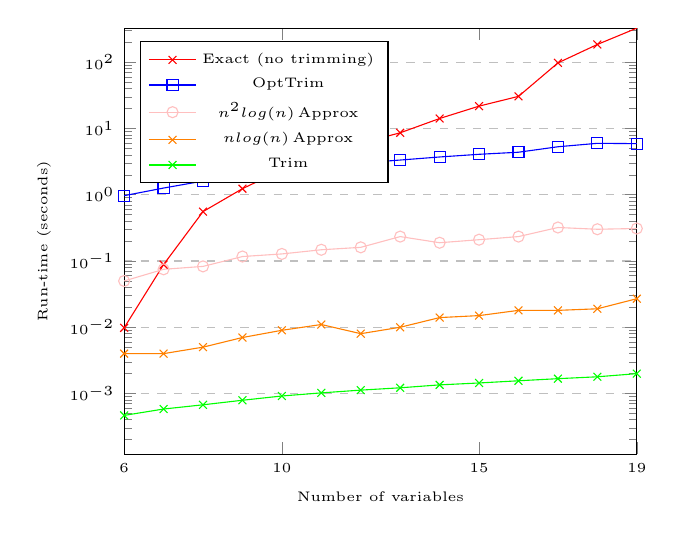
\begin{tikzpicture}
	\begin{axis}[
	scale=.95,
    ymode=log,
	xlabel={Number of variables},
	ylabel={Run-time (seconds)},
	xmin=6, xmax=19,
	ymin=0, ymax=327,
	xtick={6,10,15,19},
	legend pos=north west, style={font=\tiny\selectfont},
	ymajorgrids=true,
	grid style=dashed,
	]
	
	\addplot[
	color=red,
	mark=x,
	]
	coordinates {
		(6  , 0.00977492332458)
		(7  , 0.0880949497223)
		(8  , 0.556006193161)
		(9  , 1.23386096954)
		(10 , 2.37807798386)
		(11 , 4.2376730442)
		(12 , 6.03167200089)
		(13 , 8.61568593979)
		(14 , 14.1664741039)
		(15 , 21.7874569893)
		(16 , 30.5902190208)
		(17 , 97.9485061169)
		(18, 186.025614977) 
		(19, 327.884781122) 
	};
	\addlegendentry{Exact (no trimming)}

    \addplot[
	color=blue,
	mark=square,
	]
	coordinates { 
		(6 , 0.967791080475) 
		(7 , 1.26214194298) 
		(8 , 1.60830593109) 
		(9 , 1.97642302513) 
		(10, 2.28711390495) 
		(11, 2.67097711563) 
		(12, 3.01373195648) 
		(13, 3.3420279026) 
		(14, 3.71830201149) 
		(15, 4.08019995689) 
		(16, 4.3857190609) 
		(17, 5.30444002151)
		(18, 5.97745299339) 
		(19, 5.91222810745) 
	};
	\addlegendentry{$\OptTrim$}
	
    \addplot[
	color=pink,
	mark=o,
	]
	coordinates {
		(6  , 0.04986763000488281)
		(7  , 0.0747988224029541)
		(8  , 0.0827784538269043)
		(9  , 0.11668658256530762)
		(10 , 0.12765932083129883)
		(11 , 0.14760947227478027)
		(12 , 0.16057085990905762)
		(13 , 0.23337483406066895)
		(14 , 0.1884934902191162)
		(15 , 0.2094745635986328)
		(16 , 0.23337602615356445)
		(17 , 0.3201446533203125)
		(18, 0.3011953830718994) 
		(19, 0.3091733455657959) 
	};
	\addlegendentry{$n^2log(n) \KlmApprox$}
	
	\addplot[
	color=orange,
	mark=x,
	]
	coordinates {
		(6  , 0.003989458084106445)
		(7  , 0.00398707389831543)
		(8  , 0.004992485046386719)
		(9  , 0.006980419158935547)
		(10 , 0.008974790573120117)
		(11 , 0.010970354080200195)
		(12 , 0.007979631423950195)
		(13 , 0.00997161865234375)
		(14 , 0.013960838317871094)
		(15 , 0.014958381652832031)
		(16 , 0.017947673797607422)
		(17 , 0.017951011657714844)
		(18, 0.018949508666992188) 
		(19, 0.026926517486572266) 
	};
	\addlegendentry{$nlog(n) \KlmApprox$}
    
	
	\addplot[
	color=green,
	mark=x,
	]
	coordinates {
		(6  , 0.000465154647827)
		(7  , 0.000580787658691)
		(8  , 0.000672817230225)
		(9  , 0.000787973403931)
		(10 , 0.000914096832275)
		(11 , 0.00101804733276)
		(12 , 0.00112104415894)
		(13 , 0.0012149810791)
		(14 , 0.00134491920471)
		(15 , 0.00143694877625)
		(16 , 0.00155091285706)
		(17 , 0.00166893005371)
		(18 , 0.00178194046021)
		(19 , 0.00198793411255)
	};
	\addlegendentry{$\Trim$}
	\end{axis}
	\end{tikzpicture}
	\caption{Run-time of a long computation with $\OptTrim$, with $\Trim$, and without any trimming (exact computation).}
	\label{fig:runtime}
\end{figure}
\paragraph{Single step support minimisation.}
In order to better understand the quality gaps in practice between $\KlmApprox$, $\OptTrim$, and $\Trim$, we tested their relative errors when applied on single random variables with support size $n = 100$, and different $m$s. Note that the error obtained by $\KlmApprox$ is optimal while the other methods are not optimised for the Kolmogorv distance. In each instance of this experiment, a random variable is randomly generated by choosing the probabilities of each element in the support uniformly and then normalising these probabilities so that they sum to one.

Figure~\ref{fig:error} presents the error produced by the above methods. The depicted results are averages over fifty instances of random variables. The curves in the figure show the average error of $\OptTrim$ and $\Trim$ operators with comparison to the average error of the optimal approximation provided by $\KlmApprox$ as a function of $m$. It is evident from this graphs that increasing the support size of the approximation $m$ reduces the error, as expected, in all three methods. However, the (optimal) errors produced by the $\KlmApprox$ are significantly smaller, a half of the error produced by $\OptTrim$ and $\Trim$.


\begin{figure}[htb]
	\scriptsize	
	\centering 
	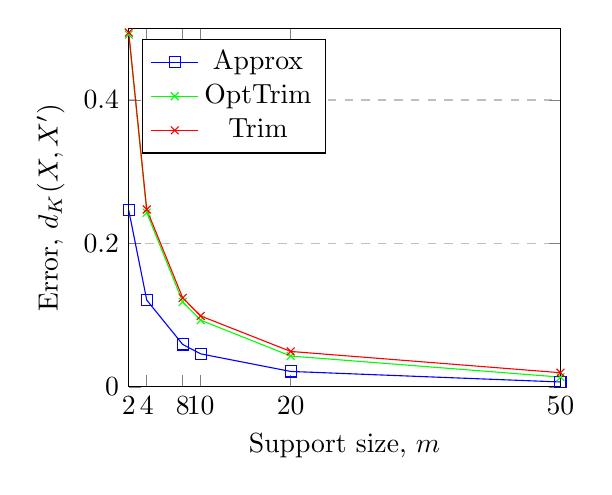
\begin{tikzpicture}
	\begin{axis}[
	scale=.8,
	xlabel={Support size, $m$},
	ylabel={Error, $d_K(X,X')$},
	xmin=2, xmax=50,
	ymin=0, ymax=0.5,
	xtick={2,4,8,10,20,50},
	legend pos=north west,
	ymajorgrids=true,
	grid style=dashed,
	]
	
	\addplot[
	color=blue,
	mark=square,
	]
	coordinates { 
		(2 , 0.246) 
		(4 , 0.121) 
		(8 , 0.0591) 
		(10 , 0.046) 
		(20, 0.0215) 
		(50, 0.0068) 
		
	};
	\addlegendentry{$\KlmApprox$}
	
	\addplot[
	color=green,
	mark=x,
	]
	coordinates {
		(2 , 0.491) 
		(4 , 0.2428) 
		(8 , 0.1184) 
		(10 , 0.0929) 
		(20, 0.0430) 
		(50, 0.0136) 
	};
	\addlegendentry{$\OptTrim$}
	
	\addplot[
	color=red,
	mark=x,
	]
	coordinates {
		(2 , 0.494) 
		(4 , 0.2473) 
		(8 , 0.124) 
		(10 , 0.0988) 
		(20, 0.0494) 
		(50, 0.01971)  
	};
	\addlegendentry{$\Trim$}
	
	\end{axis}
	\end{tikzpicture}
	\caption{Error comparison between $\KlmApprox$, $\OptTrim$, and $\Trim$ on randomly generated random variables as function of $m$.}
	\label{fig:error}
\end{figure}

% \paragraph{Comparison to Linear Programming.}
% We also compared the run-time of $\KlmApprox$ with a linear programing (LP) algorithm that also guarantees optimality, as described and discussed for example in~\cite{pavlikov2016cvar}.
% For that, we used the ``Minimize'' function of Wolfram Mathematica as a  state-of-the-art implementation of linear programing, encoding the problem by the LP problem $\min_{\alpha \in \mathbb{R}^n} \| x - \alpha\|_\infty$ subject to $\|\alpha\|_0 \leq m$ and $\| \alpha \|_1 =1$.
% The run-time comparison results were clear and persuasive: $\KlmApprox$ significantly outperforms the LP algorithm. For a random variable with support size $n=10$ and $m=5$, the LP algorithm run-time was $850$ seconds, where the $\KlmApprox$ algorithm run-time was less than a tenth of a second. For $n=100$ and $m=5$, the $\KlmApprox$ algorithm run-time was 0.14 seconds and the LP algorithm took more than a day. 
% Since it is not trivial to formally analyze the run-time of the LP algorithm, we conclude by the reported experiment that in this case the LP algorithm might not be as efficient as $\KlmApprox$ algorithm whose complexity is proven to be polynomial in Theorem~\ref{the:complexity}.

\section{Discussion and future work}\label{sec:discussion}
%Compact representations of distributions is mentioned in the literature in various contexts for various applications. In this paper, we are interested in finding optimal approximation of a random variables under the Kolmogorov metric which we define as optimal $m$-approximation. In order to achieve this optimal approximation two steps were taken, find the support of the optimal random variable and then calculate the pmf of each and every value in that support to minimize the error. Proofs of existences, optimality and run-time were detailed in Section~\ref{sec:alg} and the main algorithm was presented, the $\KlmApprox$ algorithm. Establishing the main contribution of this paper which is to present an optimal approximation scheme and to show it can be achieved in polynomial run-time. Furthermore, empirical evaluation was conducted on different domains and application to examine the algorithm performance in practice. We were interested in two aspects of performance - accuracy and run-time. Regarding to accuracy, as expected, the suggested $\KlmApprox$ algorithm results much smaller error compared to the other methods, sometimes, in more then factor 0f 2. Regarding to run-time, $\KlmApprox$ algorithm run-time is significantly much faster then LP approach. However, compared to other approximation methods accuracy vs. run-time is a trade off yet to be examined. Another interesting experiment that can be conducted in future work is to add the presented approach as one of the methods examined in~\cite{zeng2017comparison} and compare it to the binning approaches.

We developed an algorithm for computing optimal approximations of random variables where the approximation quality is measured by the Kolmogorov distance.
As demonstrated in the experiments, our algorithm improves on the approach of Cohen et al.~\cite{cohen2015estimating} and~\cite{CohenGW18} in that it finds an optimal two sided Kolmogorov approximation, and not just one sided. Beyond the Kolmogorov measure studied here we believe that similar approaches may apply also to total variation, to the Wasserstein distance, and to other measures of approximations. Another direction for future work is extensions to tables that represent other objects, not necessarily random variables. To this end, we need to extend the algorithm to support tables that do not always sum to one and tables that may contain negative entries.

\bibliographystyle{aaai}
\bibliography{library,Trim_Optimum}


\end{document}
